\documentclass[11pt,compress,t,notes=noshow, xcolor=table]{beamer}
\usepackage[]{graphicx}\usepackage[]{color}
% maxwidth is the original width if it is less than linewidth
% otherwise use linewidth (to make sure the graphics do not exceed the margin)
\makeatletter
\def\maxwidth{ %
  \ifdim\Gin@nat@width>\linewidth
    \linewidth
  \else
    \Gin@nat@width
  \fi
}
\makeatother

\newcommand{\citebutton}[2]{%
\beamergotobutton{\href{#2}{#1}}%
}

\newcommand{\blu}[1]{\textcolor{blue}{#1}}
\newcommand{\org}[1]{\textcolor{orange}{#1}}
\newcommand{\ques}{\textbf{\textcolor{red}{Question:  }}}
\newcommand{\questionssofar}{\begin{frame}\frametitle{Any questions?}\end{frame}}

\newcommand\warning{%
 \makebox[1.4em][c]{%
 \makebox[0pt][c]{\raisebox{.1em}{\scriptsize!}}%
 \makebox[0pt][c]{\color{red}\normalsize$\bigtriangleup$}}}%

\definecolor{fgcolor}{rgb}{0.345, 0.345, 0.345}
\newcommand{\hlnum}[1]{\textcolor[rgb]{0.686,0.059,0.569}{#1}}%
\newcommand{\hlstr}[1]{\textcolor[rgb]{0.192,0.494,0.8}{#1}}%
\newcommand{\hlcom}[1]{\textcolor[rgb]{0.678,0.584,0.686}{\textit{#1}}}%
\newcommand{\hlopt}[1]{\textcolor[rgb]{0,0,0}{#1}}%
\newcommand{\hlstd}[1]{\textcolor[rgb]{0.345,0.345,0.345}{#1}}%
\newcommand{\hlkwa}[1]{\textcolor[rgb]{0.161,0.373,0.58}{\textbf{#1}}}%
\newcommand{\hlkwb}[1]{\textcolor[rgb]{0.69,0.353,0.396}{#1}}%
\newcommand{\hlkwc}[1]{\textcolor[rgb]{0.333,0.667,0.333}{#1}}%
\newcommand{\hlkwd}[1]{\textcolor[rgb]{0.737,0.353,0.396}{\textbf{#1}}}%
\let\hlipl\hlkwb

\usepackage{framed}
\makeatletter
\newenvironment{kframe}{%
 \def\at@end@of@kframe{}%
 \ifinner\ifhmode%
  \def\at@end@of@kframe{\end{minipage}}%
  \begin{minipage}{\columnwidth}%
 \fi\fi%
 \def\FrameCommand##1{\hskip\@totalleftmargin \hskip-\fboxsep
 \colorbox{shadecolor}{##1}\hskip-\fboxsep
     % There is no \\@totalrightmargin, so:
     \hskip-\linewidth \hskip-\@totalleftmargin \hskip\columnwidth}%
 \MakeFramed {\advance\hsize-\width
   \@totalleftmargin\z@ \linewidth\hsize
   \@setminipage}}%
 {\par\unskip\endMakeFramed%
 \at@end@of@kframe}
\makeatother

\definecolor{shadecolor}{rgb}{.97, .97, .97}
\definecolor{messagecolor}{rgb}{0, 0, 0}
\definecolor{warningcolor}{rgb}{1, 0, 1}
\definecolor{errorcolor}{rgb}{1, 0, 0}
\newenvironment{knitrout}{}{} % an empty environment to be redefined in TeX

\usepackage{alltt}
\newcommand{\SweaveOpts}[1]{}  % do not interfere with LaTeX
\newcommand{\SweaveInput}[1]{} % because they are not real TeX commands
\newcommand{\Sexpr}[1]{}       % will only be parsed by R
\newcommand{\xmark}{\ding{55}}%


\usepackage[english]{babel}
\usepackage[utf8]{inputenc}

\usepackage{dsfont}
\usepackage{verbatim}
\usepackage{amsmath}
\usepackage{amsfonts}
\usepackage{amssymb}
\usepackage{bm}
\usepackage{csquotes}
\usepackage{multirow}
\usepackage{longtable}
\usepackage{booktabs}
\usepackage{enumerate}
\usepackage[absolute,overlay]{textpos}
\usepackage{psfrag}
\usepackage{algorithm}
\usepackage{algpseudocode}
\usepackage{eqnarray}
\usepackage{arydshln}
\usepackage{tabularx}
\usepackage{placeins}
\usepackage{tikz}
\usepackage{setspace}
\usepackage{colortbl}
\usepackage{mathtools}
\usepackage{wrapfig}
\usepackage{bm}
\usepackage{amsmath}
\usepackage{pifont}

\usetikzlibrary{shapes.multipart,shapes,arrows,automata,positioning,calc,chains,trees, shadows}
\tikzset{
  %Define standard arrow tip
  >=stealth',
  %Define style for boxes
  punkt/.style={
    rectangle,
    rounded corners,
    draw=black, very thick,
    text width=6.5em,
    minimum height=2em,
    text centered},
  % Define arrow style
  pil/.style={
    ->,
    thick,
    shorten <=2pt,
    shorten >=2pt,}
}

\tikzstyle{vec}=[draw, rectangle, fill = white, minimum width=5mm, minimum height=1cm, inner sep = 2pt]

\usepackage{subfig}

% Defines macros and environments
\usepackage{../../style/lmu-lecture}


\let\code=\texttt
\let\proglang=\textsf

\setkeys{Gin}{width=0.9\textwidth}

\setbeamertemplate{frametitle}{\expandafter\uppercase\expandafter\insertframetitle}

\usepackage{bbm}
% basic latex stuff
\newcommand{\pkg}[1]{{\fontseries{b}\selectfont #1}} %fontstyle for R packages
\newcommand{\lz}{\vspace{0.5cm}} %vertical space
\newcommand{\dlz}{\vspace{1cm}} %double vertical space
\newcommand{\oneliner}[1] % Oneliner for important statements
{\begin{block}{}\begin{center}\begin{Large}#1\end{Large}\end{center}\end{block}}


%new environments
\newenvironment{vbframe}  %frame with breaks and verbatim
{
 \begin{frame}[containsverbatim,allowframebreaks]
}
{
\end{frame}
}

\newenvironment{vframe}  %frame with verbatim without breaks (to avoid numbering one slided frames)
{
 \begin{frame}[containsverbatim]
}
{
\end{frame}
}

\newenvironment{blocki}[1]   % itemize block
{
 \begin{block}{#1}\begin{itemize}
}
{
\end{itemize}\end{block}
}

\newenvironment{fragileframe}[2]{  %fragile frame with framebreaks
\begin{frame}[allowframebreaks, fragile, environment = fragileframe]
\frametitle{#1}
#2}
{\end{frame}}


\newcommand{\myframe}[2]{  %short for frame with framebreaks
\begin{frame}[allowframebreaks]
\frametitle{#1}
#2
\end{frame}}

\newcommand{\remark}[1]{
  \textbf{Remark:} #1
}


\newenvironment{deleteframe}
{
\begingroup
\usebackgroundtemplate{
\includegraphics[width=\paperwidth,height=\paperheight]{../style/color/red.png}}
 \begin{frame}
}
{
\end{frame}
\endgroup
}
\newenvironment{simplifyframe}
{
\begingroup
\usebackgroundtemplate{
\includegraphics[width=\paperwidth,height=\paperheight]{../style/color/yellow.png}}
 \begin{frame}
}
{
\end{frame}
\endgroup
}\newenvironment{draftframe}
{
\begingroup
\usebackgroundtemplate{
\includegraphics[width=\paperwidth,height=\paperheight]{../style/color/green.jpg}}
 \begin{frame}
}
{
\end{frame}
\endgroup
}
% https://tex.stackexchange.com/a/261480: textcolor that works in mathmode
\makeatletter
\renewcommand*{\@textcolor}[3]{%
  \protect\leavevmode
  \begingroup
    \color#1{#2}#3%
  \endgroup
}
\makeatother





\input{../../latex-math/basic-math.tex}
\input{../../latex-math/basic-ml.tex}

\newcommand{\titlefigure}{figure/elmo.jpg}
\newcommand{\learninggoals}{
\item Understand the contextualization of word embeddings
\item Get the intuition of feature-based Transfer Learning}

\title{Deep Learning Basics}
% \author{}
\institute{\href{https://slds-lmu.github.io/lecture_dl4nlp/}{slds-lmu.github.io/lecture\_dl4nlp}}
\date{}

\begin{document}
\lecturechapter{ELMo \beamergotobutton{\href{https://aclanthology.org/N18-1202/}{Peters et al., 2018}}}
\lecture{Deep Learning for NLP}

% ------------------------------------------------------------------------------

\begin{vbframe}{Recap: Word vectors}

\vfill

	\begin{figure}
		\centering
		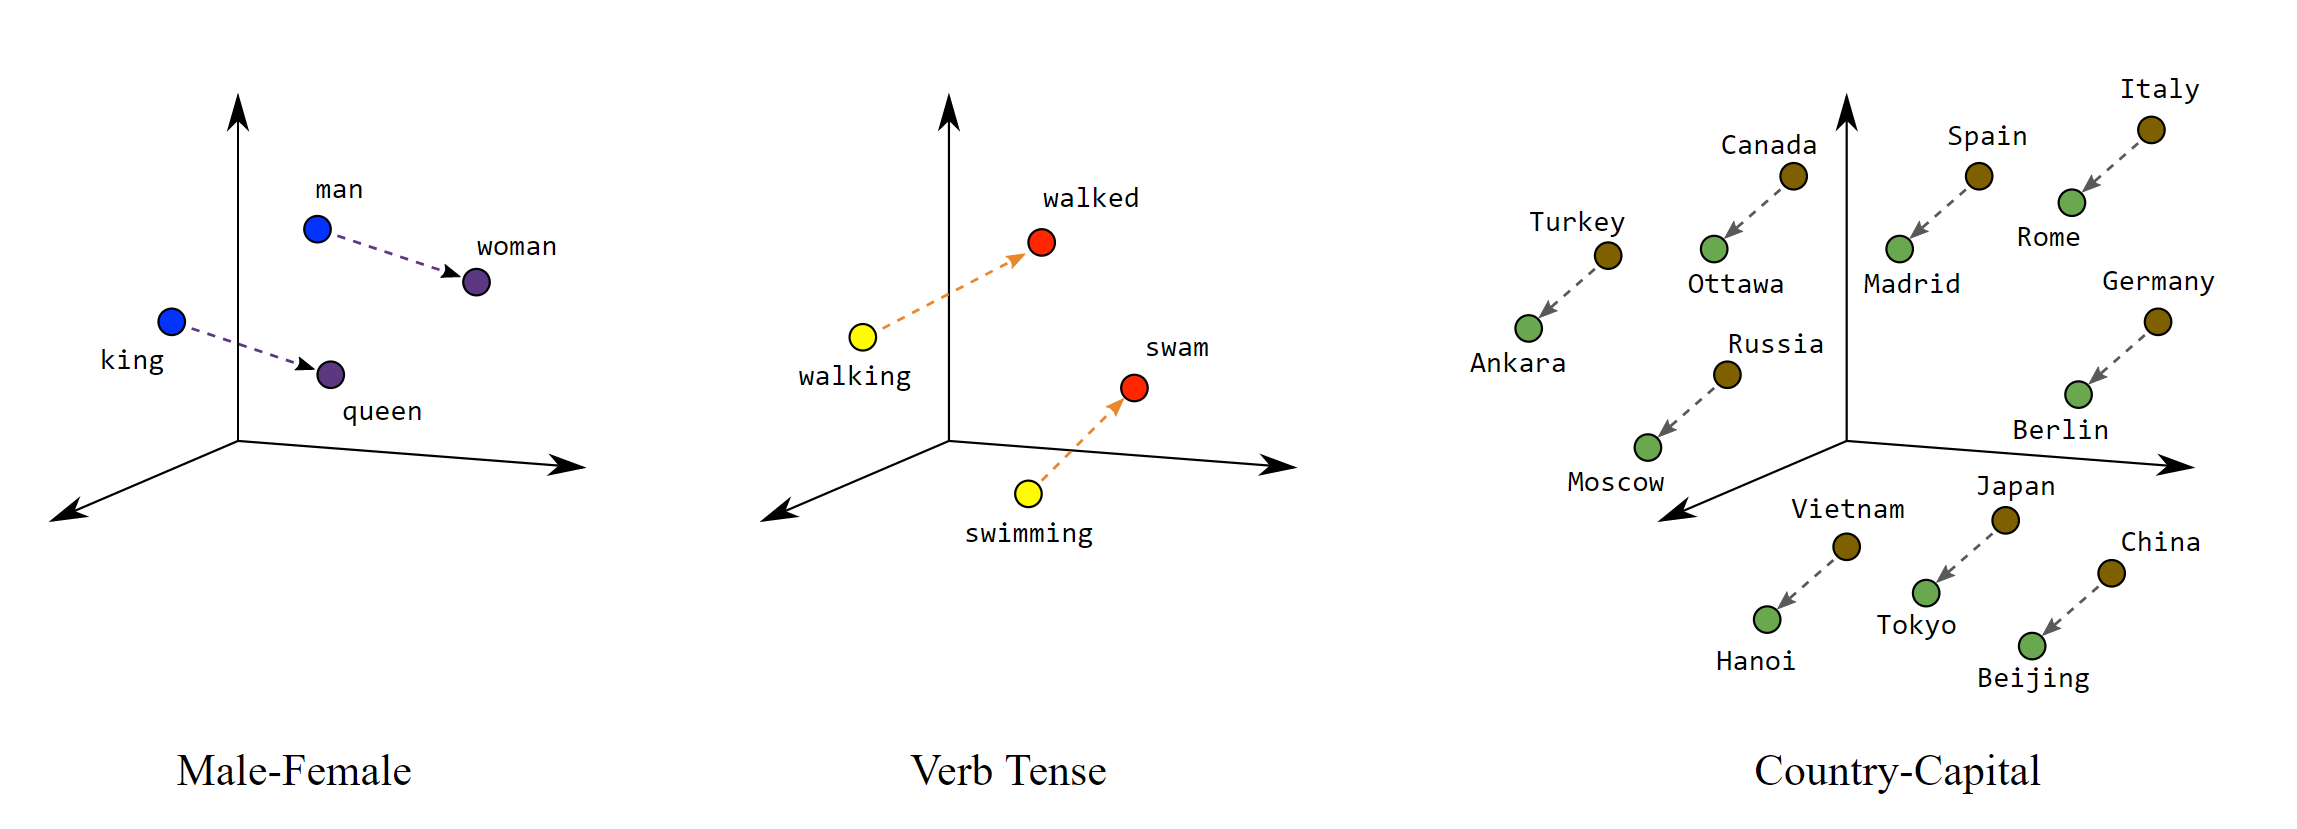
\includegraphics[width = 11cm]{figure/linear-relationships.png}\\ 
		\beamergotobutton{\href{https://developers.google.com/machine-learning/crash-course/embeddings/translating-to-a-lower-dimensional-space}{Source: Google}}
	\end{figure}

	\begin{itemize}
		\item Information is encoded in (pre-)trained word embeddings
		\item Embeddings are used for tasks external to the training corpus
	\end{itemize}

\vfill

\end{vbframe}

% ------------------------------------------------------------------------------

%\begin{vbframe}{Feature-based Transfer Learning}

%\vfill

%\textbf{Using word2vec:}
	
%	\begin{enumerate}
%		\item Self-supervised pre-training of word2vec ..
%			\begin{itemize}
%				\item Using a large, unannotated corpus
%				\item Objective: CBOW or Skip-gram
%			\end{itemize}
%		.. and extract the stored knowledge (i.e. embedding)\\
%		\item \textit{Alternative:} Download embeddings from the web,
%		e.g. \url{https://code.google.com/archive/p/word2vec/}
%		\item Perform a (supervised) task using the embeddings,
%		e.g. Sentiment classification using an LSTM network
%	\end{enumerate}
	
%\textit{The stored knowledge from the pre-trained model is extracted as is
%and is not further adapted to the actual domain/task of interest!}

%\vfill

%\end{vbframe}

% ------------------------------------------------------------------------------

\begin{vbframe}{Contextuality}

\vfill

\textbf{1st Generation of neural embeddings are "context-free":}

	\begin{itemize}
		\item Breakthrough paper (word2vec): \beamergotobutton{\href{https://arxiv.org/abs/1301.3781}{Mikolov et al, 2013}}
		\item Followed by GloVe: \beamergotobutton{\href{https://aclanthology.org/D14-1162/}{Pennington et al, 2014}}
		\item FastText as extension of word2vec: \beamergotobutton{\href{https://arxiv.org/abs/1607.04606}{Bojanowski et al, 2016}}
	\end{itemize}
	
	\textbf{Why "Context-free"?}
	
	\begin{itemize}
		\item Models learn \textit{one single} embedding for each word
		\item Why could this possibly be problematic?
			\begin{itemize}
				\item "The \textit{default} setting of the function is xyz."
				\item "The probability of \textit{default} is rather high."
			\end{itemize}
		\item Would be nice to have different embeddings for these two occurrences
	\end{itemize}
	
\vfill

\end{vbframe}

% ------------------------------------------------------------------------------

\begin{vbframe}{Contextual embeddings}

\vfill

	\begin{figure}
		\centering
		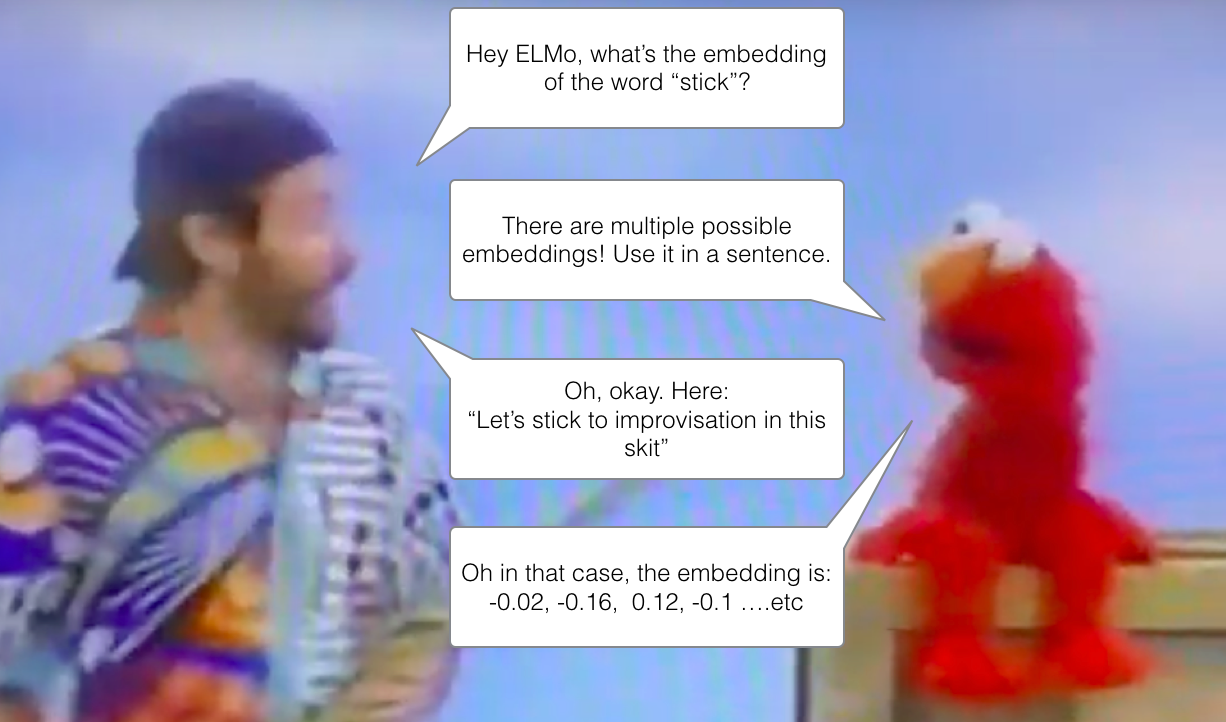
\includegraphics[width = 10cm]{figure/elmo-embedding-robin-williams.png}\\ 
		\beamergotobutton{\href{https://jalammar.github.io/illustrated-bert/}{Source: Jay Alammar}}
	\end{figure}

\vfill

\end{vbframe}

% ------------------------------------------------------------------------------

\begin{vbframe}{embeddings from language models}

\vfill

\begin{itemize}
		\item Bidirectional language model (LM)
		\item Combines a forward LM $$p\left(w_{1}, w_{2}, \ldots, w_{N}\right)=\prod_{k=1}^{N} p\left(w_{k} | w_{1}, w_{2}, \ldots, w_{k-1}\right)$$
					and a backward LM $$p\left(w_{1}, w_{2}, \ldots, w_{N}\right)=\prod_{k=1}^{N} p\left(w_{k} | w_{k+1}, w_{k+2}, \ldots, w_{N}\right)$$
					to arrive at the following loglikelihood:
					$$\begin{array}{l}
\sum_{k=1}^{N}\left(\log p\left(w_{k} | w_{1}, \ldots, w_{k-1} ; \Theta_{x}, \overrightarrow{\Theta}_{L S T M}, \Theta_{s}\right)\right. \\
\quad\left. +\log p\left(w_{k} | w_{k+1}, \ldots, w_{N} ; \Theta_{x}, \overleftarrow{\Theta}_{L S T M}, \Theta_{s}\right)\right)
\end{array}$$
	\end{itemize}

\vfill

\end{vbframe}

% ------------------------------------------------------------------------------

\begin{vbframe}{ELMo embeddings}

\vfill

	\begin{itemize}
		\item Character-based (context-independent) token representations $$\vec x_k^{LM}$$
		\item Two-layer biLSTM as main architecture:
			\begin{itemize}
				\item Two context-dependent token representations \textit{per layer}, i.e.
							$$\overrightarrow{\vec h}_{k, j}^{L M}\; \mbox{\&}\; \overleftarrow{\vec h}_{k, j}^{L M}\; \mbox{for the $k$-th token in the $j$-th layer.}$$
				\item Four context-dependent token representations in total: 
							$$\left\{\overrightarrow{\vec h}_{k, j}^{L M}, \overleftarrow{\vec h}_{k, j}^{L M} | j = 1, 2\right\}$$
			\end{itemize}
		\item Five representations per token in total:
					$$\begin{aligned}
R_{k} &=\left\{\vec x_{k}^{L M}, \overrightarrow{\vec h}_{k, j}^{L M}, \overleftarrow{\vec h}_{k, j}^{L M} | j=1, \ldots, L\right\} \\
&=\left\{\vec h_{k, j}^{L M} | j = 0, 1, 2\right\}
\end{aligned}$$
	\end{itemize}

\vfill

\end{vbframe}

% ------------------------------------------------------------------------------

\begin{vbframe}{Graphical representation}

\vfill

	\begin{figure}
		\centering
		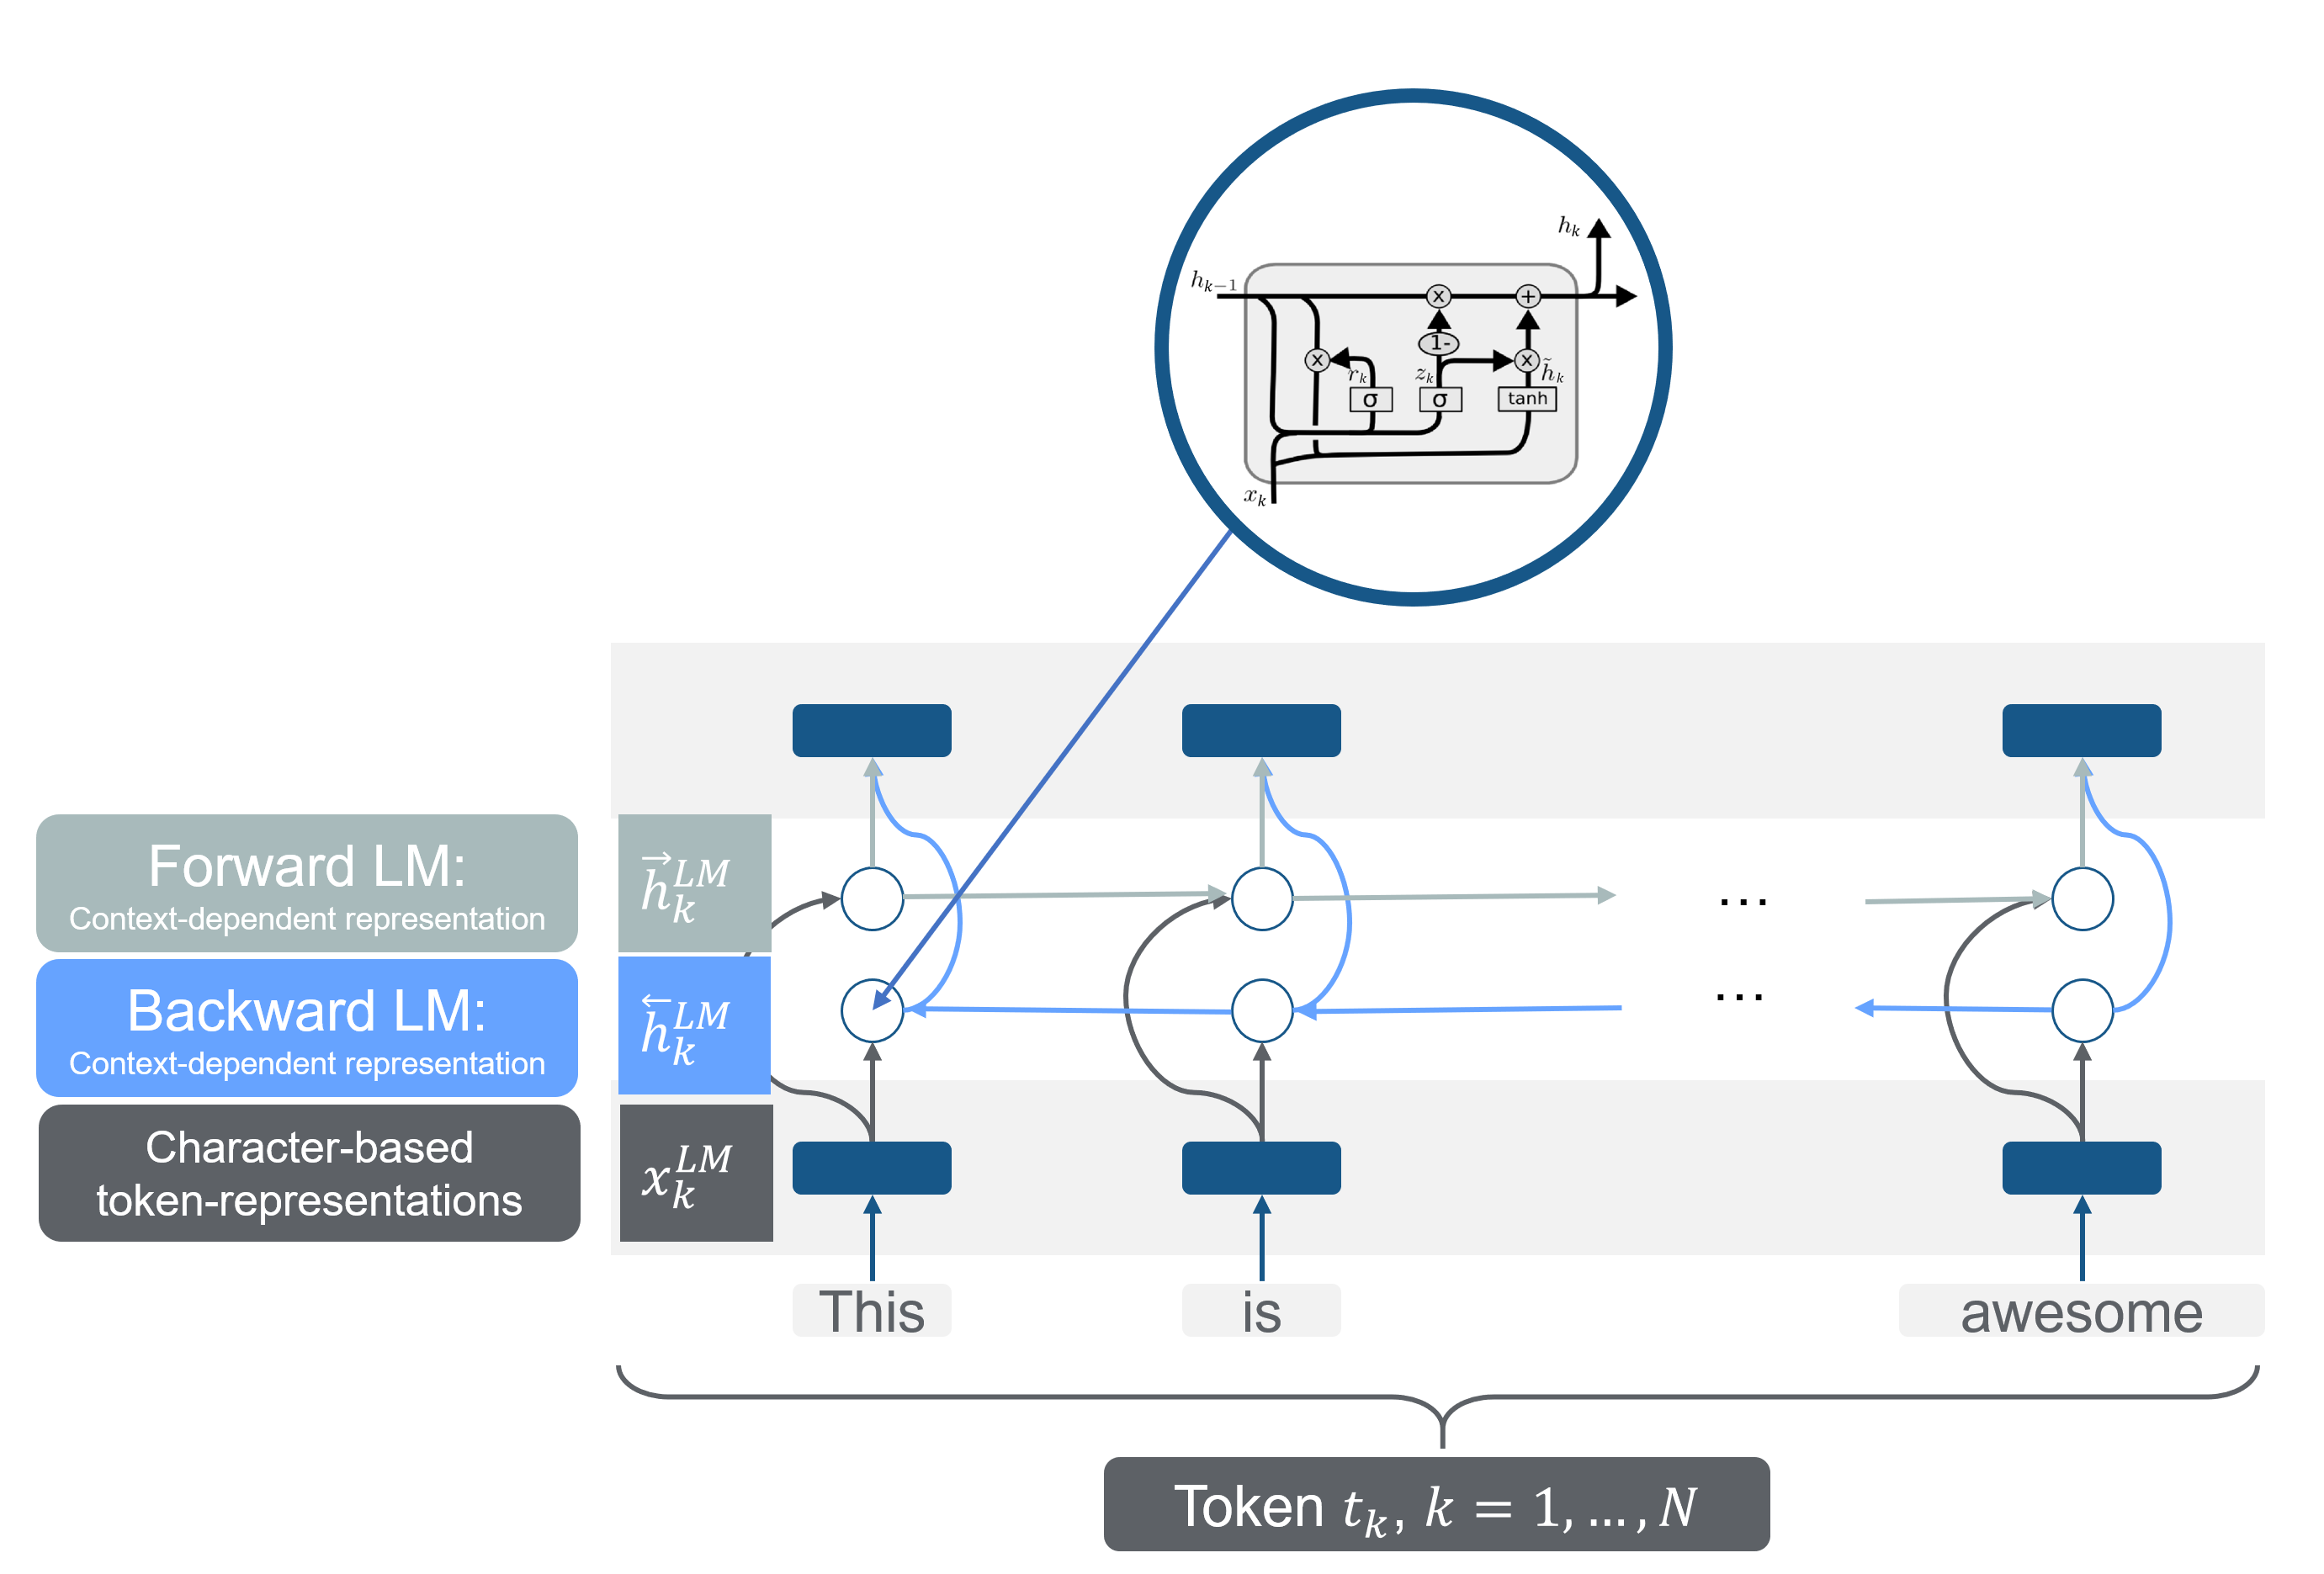
\includegraphics[width = 10cm]{figure/elmo-pretrained-bilm}\\ 
		\beamergotobutton{\href{https://slds-lmu.github.io/seminar_nlp_ss20/transfer-learning-for-nlp-i.html}{Source: Carolin Becker}}
	\end{figure}

\vfill

\end{vbframe}

% ------------------------------------------------------------------------------

\begin{vbframe}{Graphical representation}

\vfill
			
	\begin{figure}
		\centering
		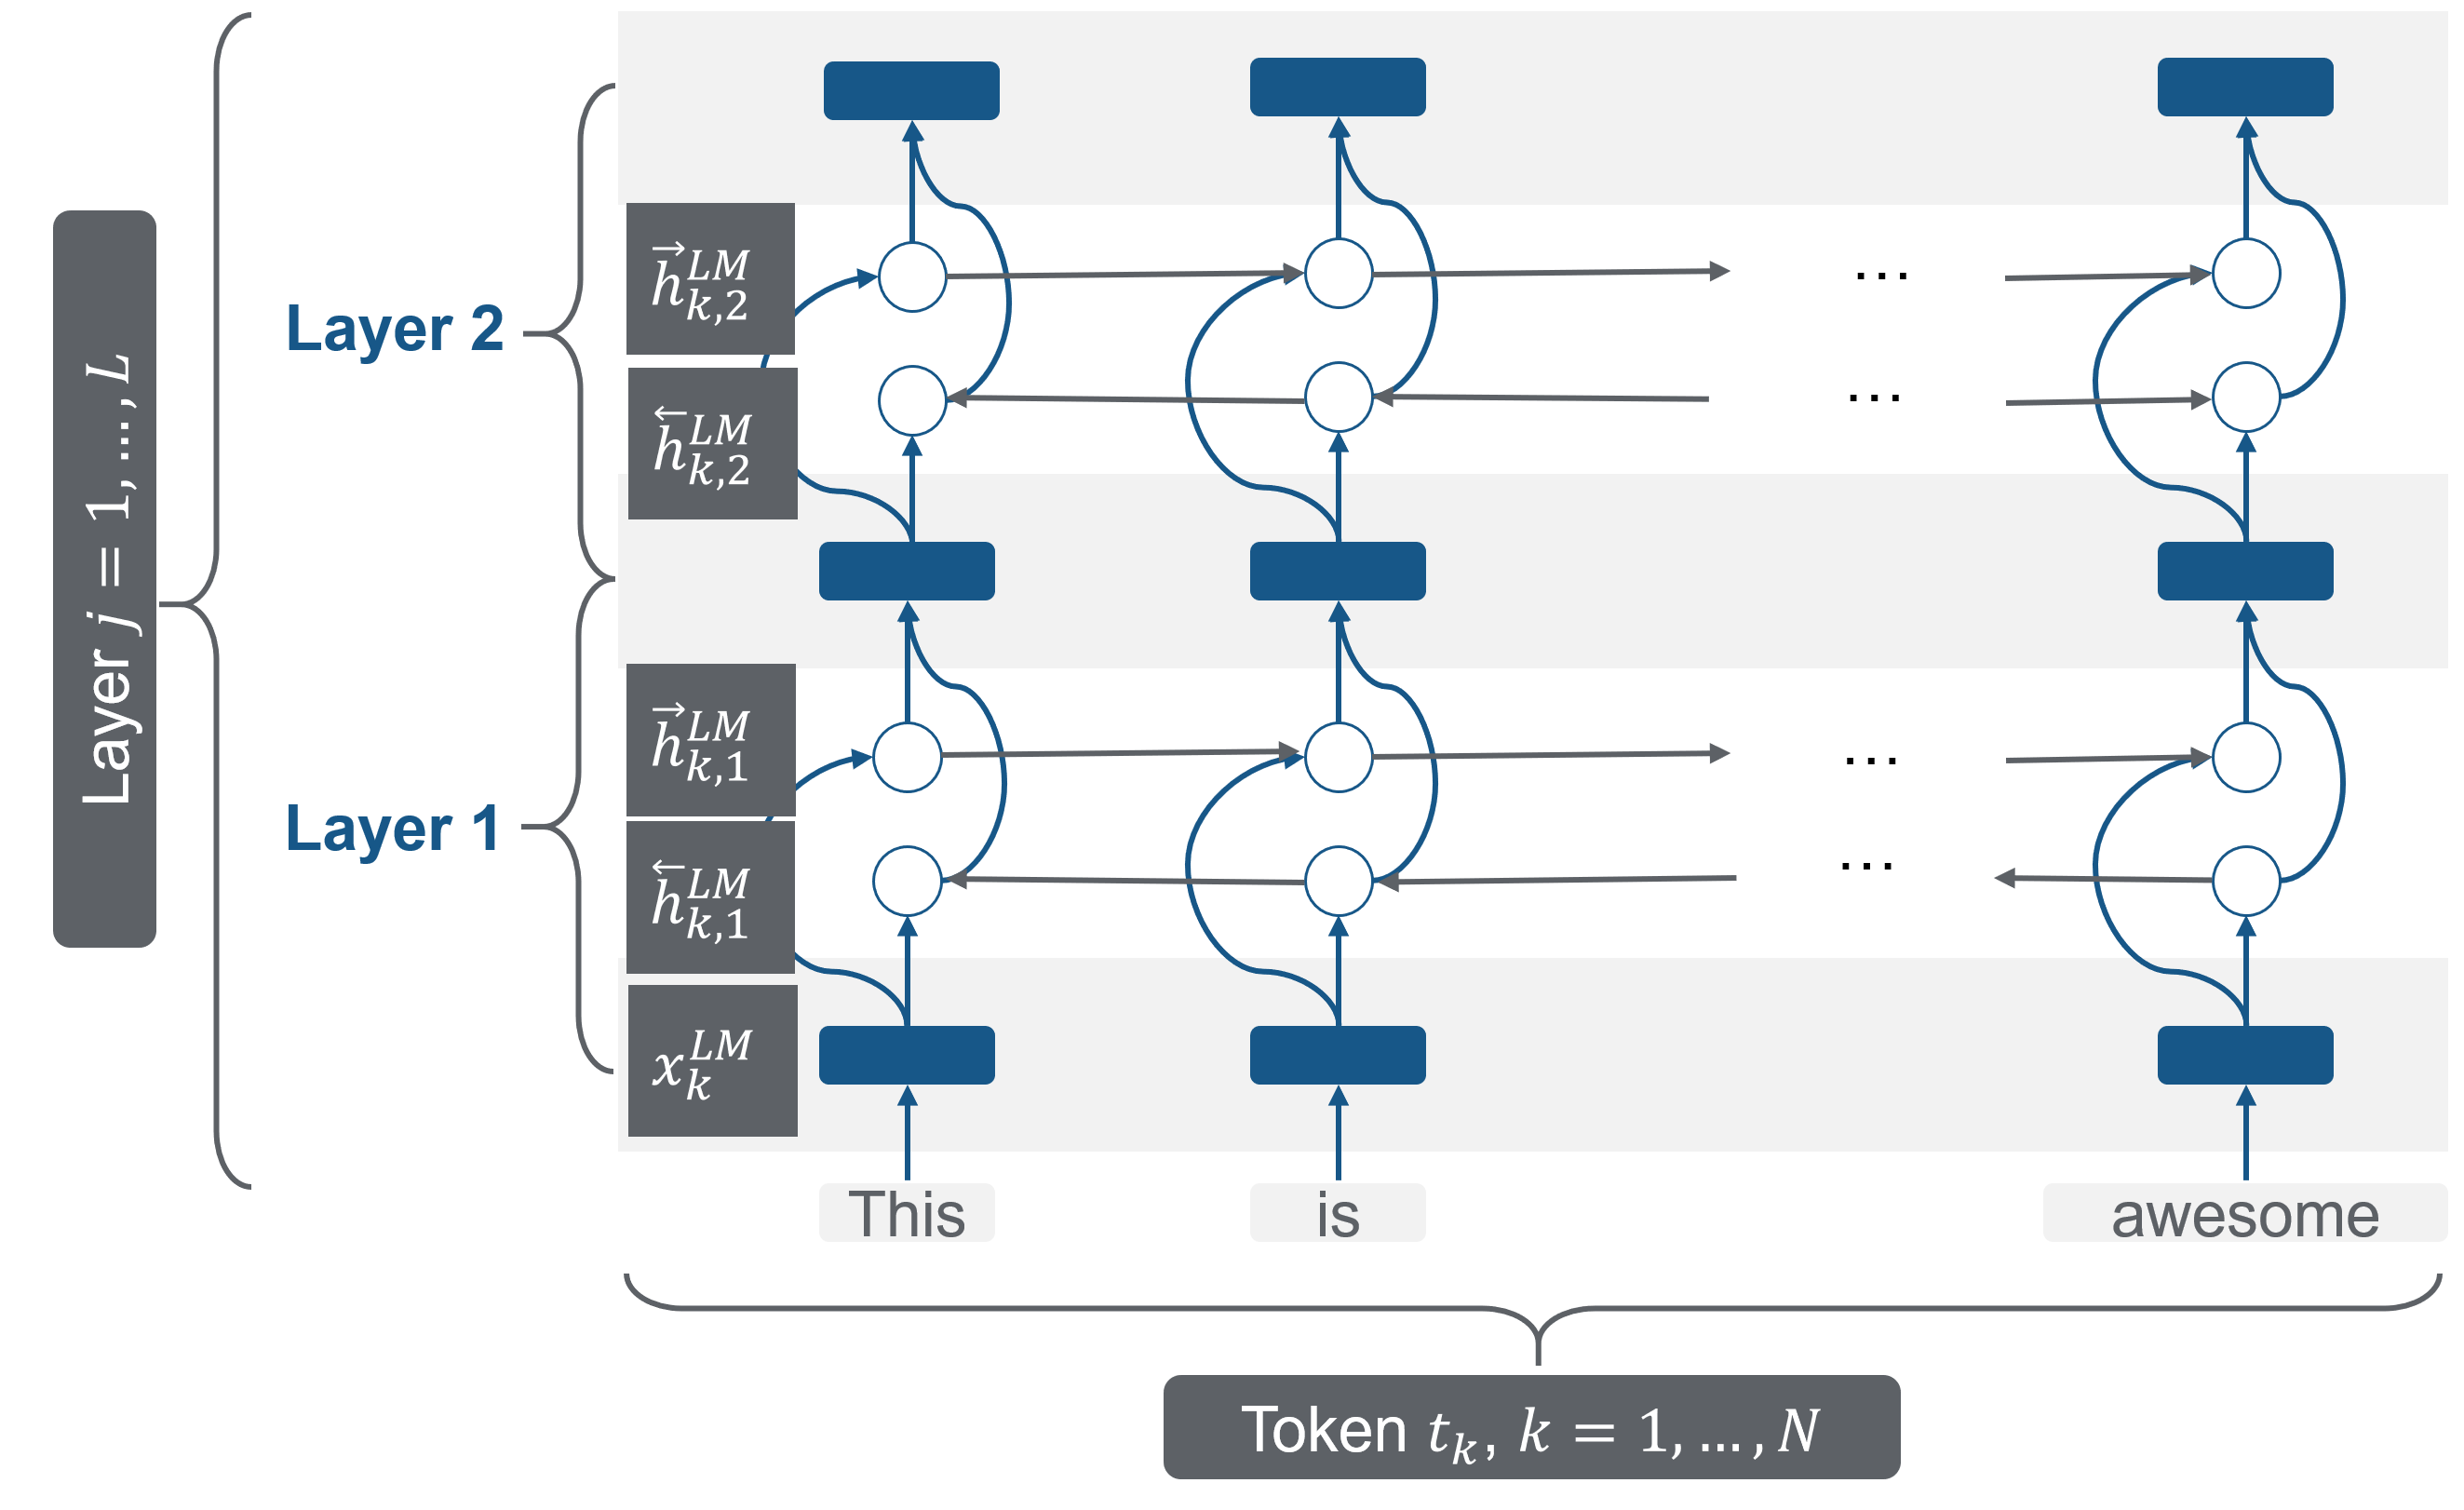
\includegraphics[width = 10cm]{figure/elmo-pretrained-bilm-2}\\ 
		\beamergotobutton{\href{https://slds-lmu.github.io/seminar_nlp_ss20/transfer-learning-for-nlp-i.html}{Source: Carolin Becker}}
	\end{figure}

\vfill

\end{vbframe}

% ------------------------------------------------------------------------------

\begin{vbframe}{Task Adaption}

\vfill

\textbf{Including ELMo in downstream tasks:}

	\begin{itemize}
		\item Calculate task-specific weights of all five representations:
					$$\mathbf{E} \mathbf{L} \mathbf{M} \mathbf{o}_{k}^{t a s k}=E\left(R_{k} ; \Theta^{t a s k}\right)=\gamma^{t a s k} \sum_{j=0}^{L} s_{j}^{t a s k} \vec h_{k, j}^{L M},$$
					where the $\vec h_{k, j}^{L M}$ are \textbf{not trainable} anymore.
		\item Trainable parameters during the adaption:
			\begin{itemize}
				\item $s_{j}^{t a s k}$ are trainable (softmax-normalized) weights
				\item $\gamma^{t a s k}$ is a trainable scaling parameter
			\end{itemize}
	\end{itemize}

	\textbf{Advantages over context free-embeddings:}

	\begin{itemize}
		\item Task-specific model has access to \textit{multiple} representations of each token
		\item Model learns to which degree to use the different representations depending on the task at hand
	\end{itemize}

\vfill

\end{vbframe}

% ------------------------------------------------------------------------------

\begin{vbframe}{Task Adaption}

\vfill

	\begin{figure}
		\centering
		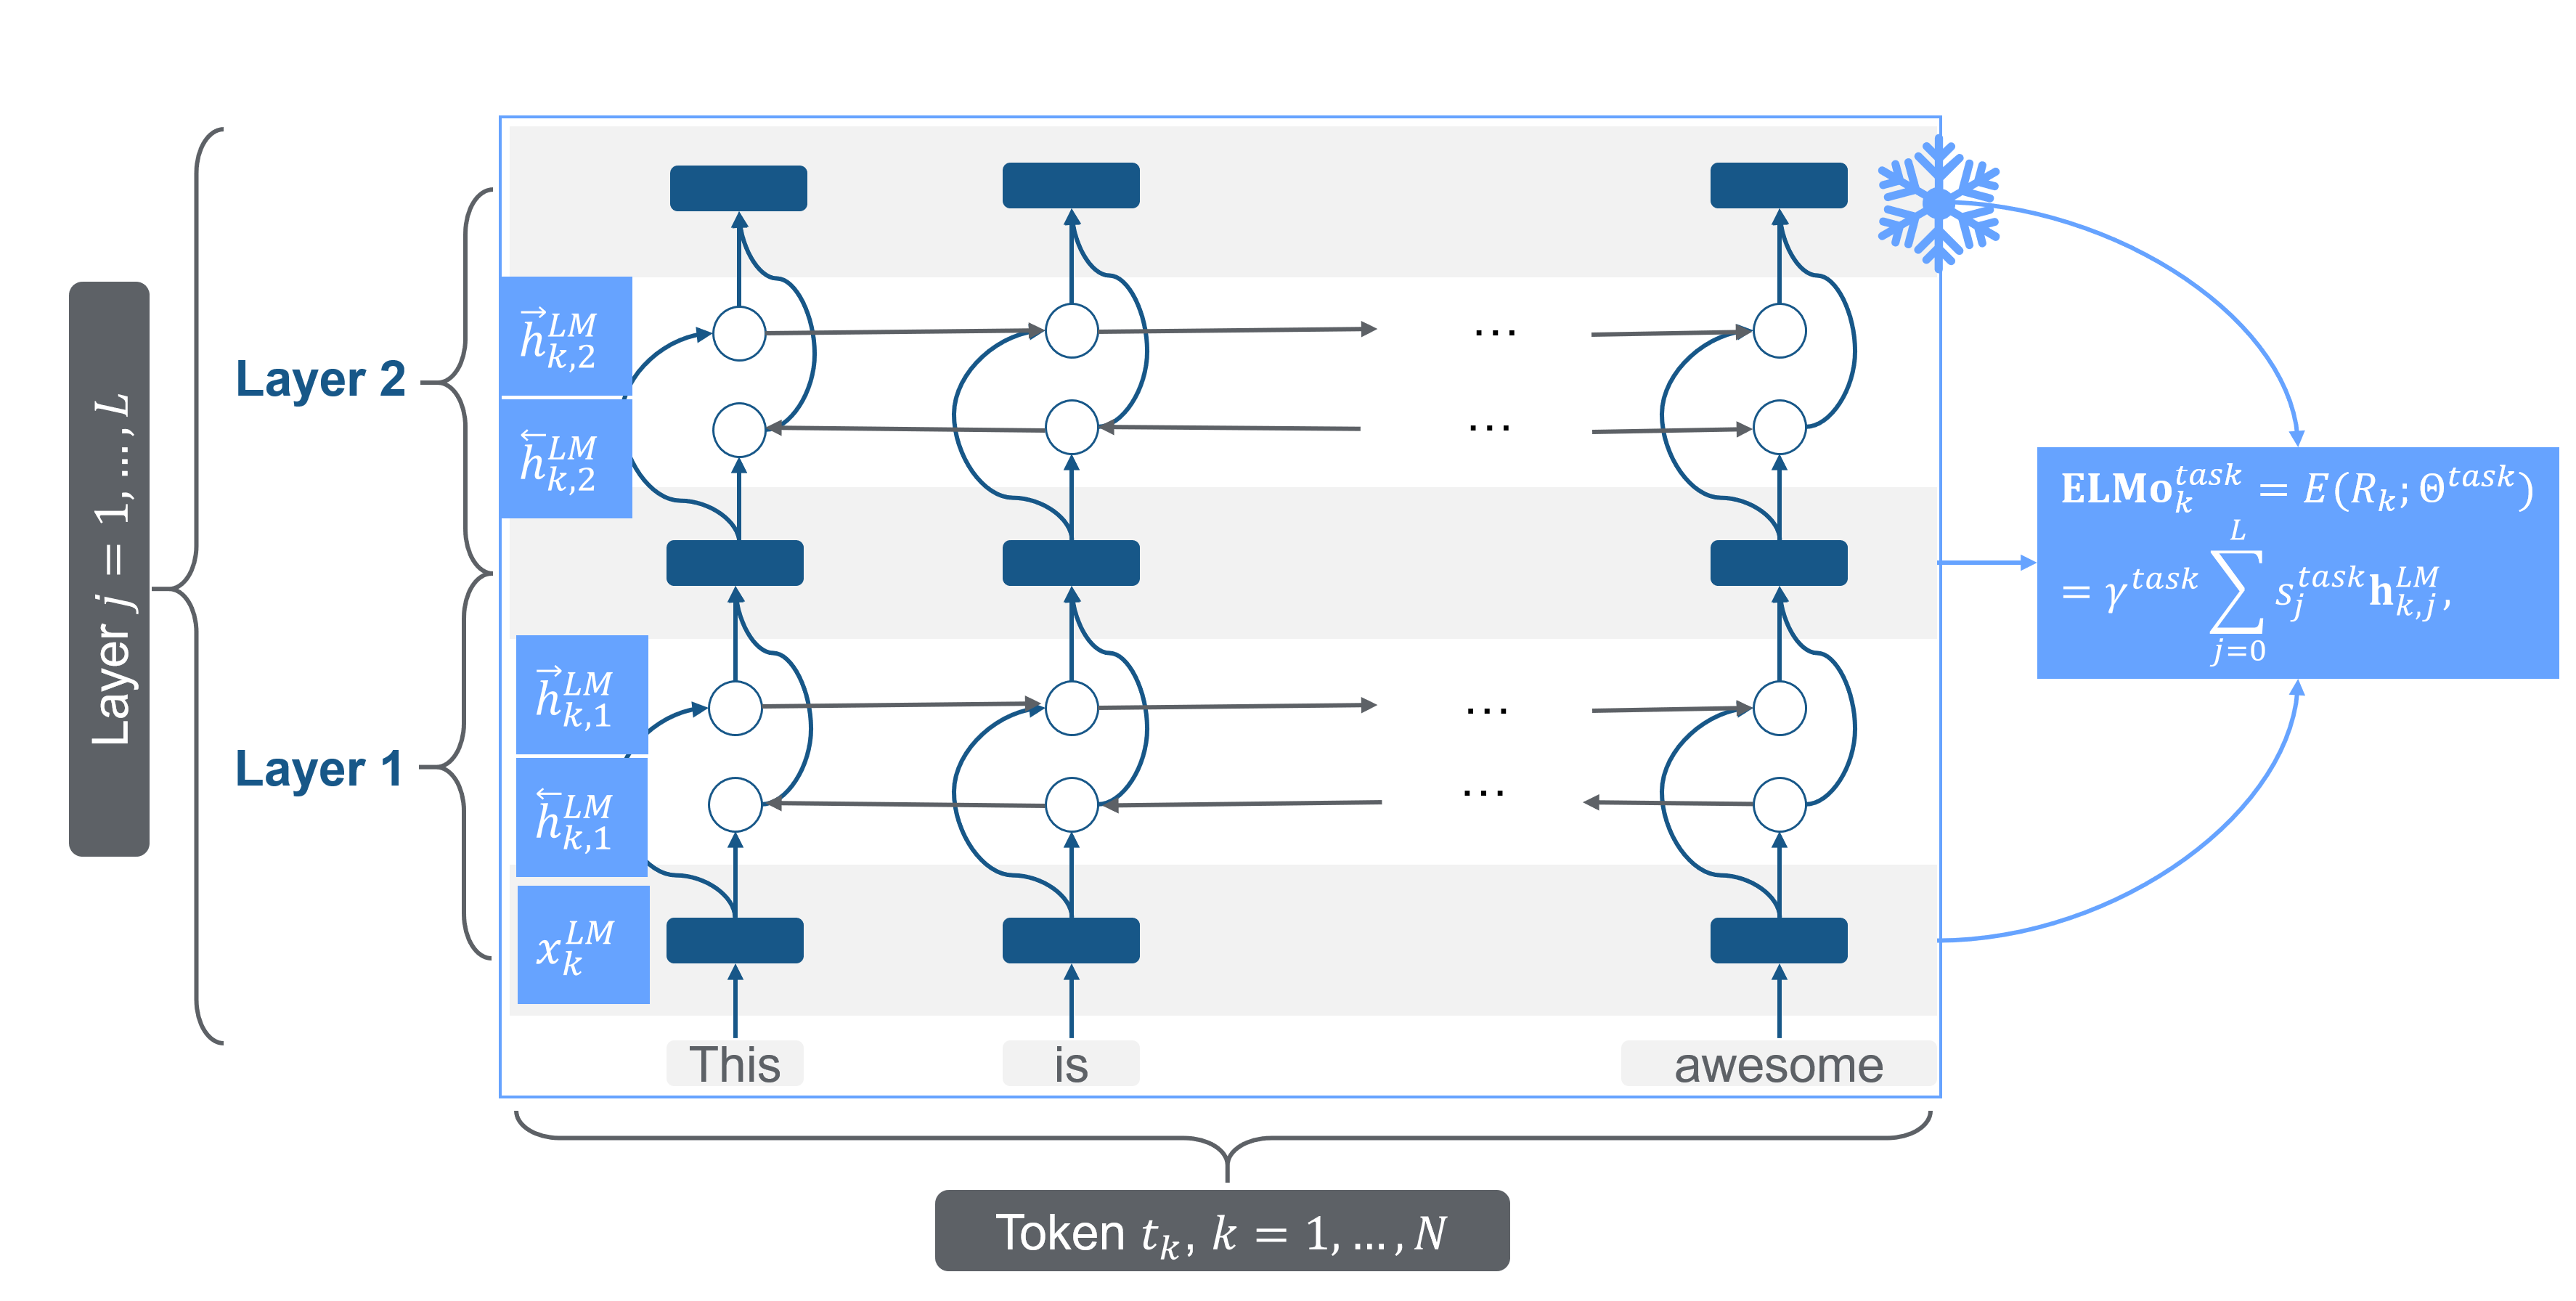
\includegraphics[width = 12cm]{figure/elmo-adaption}\\ 
		\beamergotobutton{\href{https://slds-lmu.github.io/seminar_nlp_ss20/transfer-learning-for-nlp-i.html}{Source: Carolin Becker}}
	\end{figure}

\vfill

\end{vbframe}

% ------------------------------------------------------------------------------

\begin{vbframe}{Performance}

\vfill
			
	\begin{figure}
		\centering
		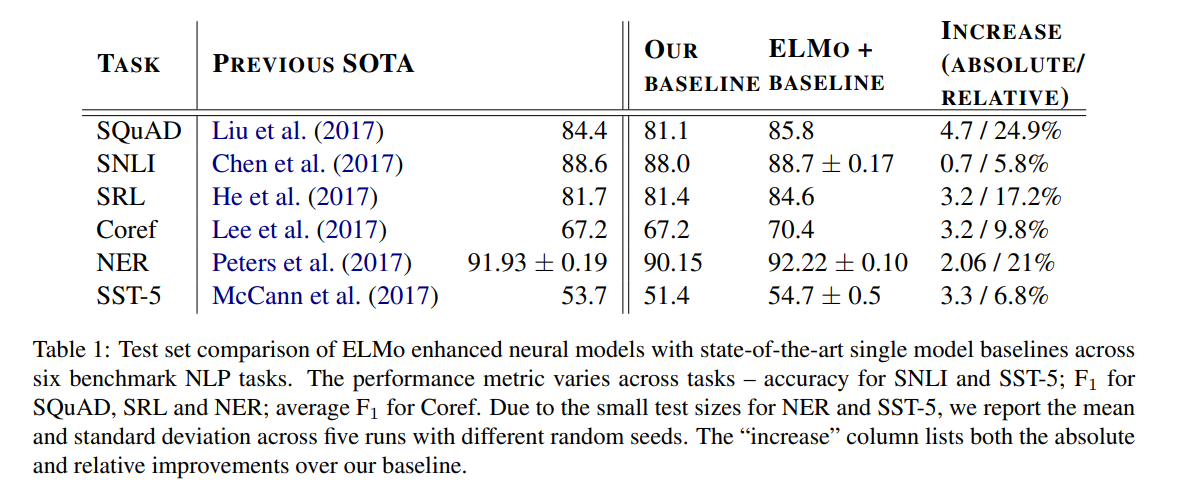
\includegraphics[width = 12cm]{figure/elmo-sota.png}\\ 
		\beamergotobutton{\href{https://aclanthology.org/N18-1202/}{Source: Peters et al., 2018}}
	\end{figure}

\vfill

\end{vbframe}

% ------------------------------------------------------------------------------

\begin{vbframe}{Summary}

\vfill

	\begin{itemize}
		\item Embeddings are (bidirectionally!) contextualized \\
					(as opposed to word2vec)
		\item Embeddings are \textit{not} adapted to target domain/task \\
					(similar as for word2vec)
		\item Additional weights are learned for each downstream task \\
					(i.e. besides the embeddings, no shared knowledge across tasks)
	\end{itemize}

\vfill

\end{vbframe}

% ------------------------------------------------------------------------------

\endlecture
\end{document}
